\section{Data and methods}\label{sec:methods}

\subsection{Data}
The repository contains three analysis tables, a locked evaluation split, and
the complete traces needed to reproduce every reported result.

\paragraph{D1: Timeline.} Twenty-seven (model, benchmark, score, date, source)
rows spanning 2018--2026, drawn from the original papers and from leaderboard
mirrors (Table~\ref{tab:timeline}; full file \texttt{data/models\_timeline.csv}).
Where multiple evaluation variants exist we record the variant explicitly
(e.g., vendor-reported vs.\ independent SWE-bench Verified).

\paragraph{D2: 2026 frontier matrix.} Per-model benchmark scores and API prices
for the July 2026 frontier --- GPT-5.6 Sol/Terra/Luna, Claude Fable~5, Claude
Opus~5, Kimi~K3, plus the April 2026 flagship GPT-5.5 and Claude Opus~4.8 ---
from OpenAI's GPT-5.6 launch tables~\cite{openai2026gpt56}, Anthropic's Opus~5
launch and system card~\cite{anthropic2026opus5,anthropic2026opus5card},
Artificial Analysis~\cite{aa2026gpt56,gist2026aa56}, the Vals AI independent
SWE-bench Verified harness~\cite{vals2026swebench}, and arena.ai's
human-preference Frontend Code Arena~\cite{arena2026webdev}.

\paragraph{D3: Pricing.} Input/output prices per million tokens for
representative API models from 2020 to 2026, using vendor documentation where
available~\cite{deploybase2026prices,openai2026gpt56}.

\paragraph{D4: Live-evaluation items.} The committed official GSM8K test split
contains 1,319 question/answer pairs~\cite{cobbe2021gsm8k}. We retain the
original 16 pilot identifiers as a locked development split and sample 100
evaluation identifiers once from the remaining rows
(\texttt{random\_state=20260810}) before v1 tuning. The split manifest records
both identifier lists and the source-parquet SHA-256 digest.

\paragraph{Provenance caveat.} Mid-2026 numbers mix vendor-reported and
independent evaluations. We label provenance wherever it matters and prefer
third-party measurements (Vals AI, Artificial Analysis, ARC Prize) when both
exist. Vendor launch numbers are claims, not independent results; we treat them
as such and note where vendor and third-party harnesses differ.

\begin{figure}[t]
\centering
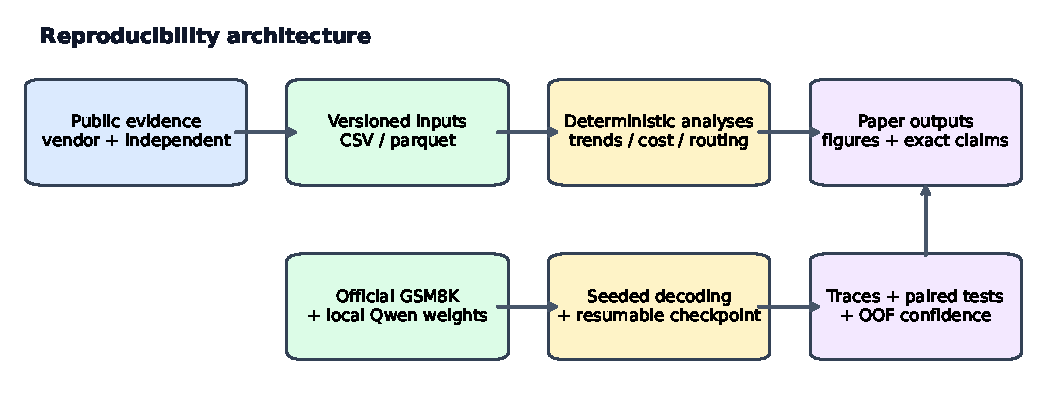
\includegraphics[width=\linewidth]{figures/architecture.pdf}
\caption{Reproducibility architecture. Public evidence feeds deterministic
trend, cost, and routing analyses. The live evaluation records complete traces
and paired statistics; the exploratory confidence stage consumes those
versioned traces. Every path produces auditable paper outputs.}\label{fig:architecture}
\end{figure}

\subsection{Analysis methods}
\paragraph{Trend fitting.} For the SWE-bench Verified series we fit a
log-linear model to the \emph{odds} of solving a task,
$\mathrm{logit}(p)$, against release date, and report the implied annual
multiplicative growth of those odds with the fit $R^2$
(Figure~\ref{fig:swe}). For MMLU we compare the raw series with the estimated
human-expert level of 89.8\%~\cite{hendrycks2021mmlu}.

\paragraph{Pareto analysis.} Using Artificial Analysis's all-effort dataset for
the GPT-5.6 family (15 model$\times$effort settings with intelligence-index
scores and per-task costs~\cite{gist2026aa56,aa2026gpt56}), we compute the
cost--capability Pareto frontier and identify dominated settings.

\paragraph{Routing oracle.} On the fourteen benchmarks that OpenAI's GPT-5.6
launch table reports for all six of Sol, Terra, Luna, GPT-5.5, Fable~5, and
Opus~4.8, we normalize each benchmark to its best model (100), then compare
(i) the best single model's mean, (ii) an oracle that picks the best model per
benchmark, and (iii) restricted routers (a cheapest-within-one-point router
and a two-model router).

\paragraph{Live experiment.} Section~\ref{sec:selfcons} describes a controlled
development/evaluation protocol. On development data we screen three prompts
(official chat-template concise, four-shot, and solve-and-check) at
temperatures 0.4 and 0.7 using Qwen2.5-0.5B-Instruct, confirm the leading
four-shot/0.4 setting on all 16 items, and compare it with
Qwen2.5-1.5B-Instruct. The primary selector is four-sample plurality; a greedy
candidate verifier is prespecified as secondary. Before evaluation, a manifest
freezes Qwen2.5-1.5B-Instruct, the official chat template with four worked
examples, $k=4$, temperature 0.4, top-$p=0.95$, seed 1234, and the plurality
selector. We then run that configuration once on all 100 disjoint evaluation
items. Every record stores the greedy completion, four sampled completions,
canonical numeric answers, prefix votes, verifier decision, and correctness.
We report exact counts, Wilson 95\% intervals, the any-sample oracle ceiling,
and two-sided exact McNemar tests against paired greedy outcomes. Atomic
checkpoints, JSONL traces, split/config hashes, and integrity tests are
provided.
\paragraph{Exploratory confidence model.} After the frozen evaluation labels
were available, we specified a simple model to estimate whether vote-at-four
was correct. Its seven reference-free features are plurality share, normalized
answer entropy, the number of distinct sampled answers, agreement of plurality
with greedy and verifier outputs, and the mean and standard deviation of
sample-completion length. We standardize these features inside each training
fold and fit an L2-regularized logistic regression. Five-fold stratified
cross-validation with shuffling and seed 20260811 yields one out-of-fold
probability for every item. We report ROC AUC, Brier score against a constant
0.62 prevalence baseline, and accuracy among the predictions retained at fixed
50\% and 75\% coverage. The features, folds, metrics, and coverage levels were
set before scoring this added analysis, but the analysis itself was designed
after the v1 outcomes were known. It is exploratory and does not constitute a
second held-out evaluation.
